\documentclass[11pt,a4paper]{article}

% -- Typography and Page Layout --
\usepackage[utf8]{inputenc}
\usepackage[T1]{fontenc}
\usepackage[expansion=false]{microtype}
\usepackage[margin=2.0cm,top=2.4cm,bottom=2.4cm]{geometry}
\usepackage{setspace}
\onehalfspacing

% -- Mathematical Packages --
\usepackage{amsmath,amssymb,amsfonts,bm,mathtools}

% -- Graphics and Color --
\usepackage{graphicx}
\usepackage[table]{xcolor}
\definecolor{navyblue}{RGB}{0, 45, 98}
\definecolor{steelcyan}{RGB}{18, 102, 140}
\definecolor{charcoal}{RGB}{35, 39, 42}
\definecolor{lightgray}{RGB}{245, 247, 250}
\definecolor{codebg}{RGB}{240, 242, 245}
\definecolor{bordercolor}{RGB}{200, 210, 220}
\definecolor{successgreen}{RGB}{16, 124, 65}
\definecolor{warnorange}{RGB}{216, 59, 1}

% -- Tables and Floats --
\usepackage{booktabs,multirow,array,tabularx,xltabular}
\usepackage{float}
\usepackage[font=small,labelfont=bf,skip=6pt]{caption}
\usepackage{subcaption}

% -- Headers and Footers --
\usepackage{fancyhdr}
\pagestyle{fancy}
\fancyhf{}
\fancyhead[L]{\small\textcolor{navyblue}{\textbf{EdgeSAR}}}
\fancyhead[R]{\small\textcolor{charcoal}{Bireysel Araştırma Projesi}}
\fancyfoot[C]{\small\thepage}
\renewcommand{\headrulewidth}{0.6pt}
\renewcommand{\footrulewidth}{0.4pt}

% -- Hyperlinks --
\usepackage{hyperref}
\hypersetup{
    colorlinks=true,
    linkcolor=navyblue,
    citecolor=navyblue,
    filecolor=navyblue,
    urlcolor=steelcyan,
   % pdfauthor={Tunahan},
    pdftitle={EdgeSAR: Sentetik Verilerle Uçtan Uca SAR Görüntü Odaklama ve Hafif Sıklet Hedef Sınıflandırma},
    pdfkeywords={SAR, Range-Doppler Algoritması, Ghost-ECANet, CA-CFAR, Grad-CAM, Gömülü Sistemler, Sinyal İşleme}
}

% -- Code Listings --
\usepackage{listings}
\lstset{
    backgroundcolor=\color{codebg},
    basicstyle=\ttfamily\footnotesize\color{charcoal},
    breaklines=true,
    captionpos=b,
    frame=single,
    rulecolor=\color{bordercolor},
    keywordstyle=\color{navyblue}\bfseries,
    commentstyle=\color{steelcyan}\itshape,
    stringstyle=\color{warnorange},
    numbers=none,
    tabsize=2
}

% -- Section Styling --
\usepackage{titlesec}
\titleformat{\section}{\Large\bfseries\color{navyblue}}{\thesection}{1em}{}[\titlerule]
\titleformat{\subsection}{\large\bfseries\color{steelcyan}}{\thesubsection}{1em}{}
\titleformat{\subsubsection}{\normalsize\bfseries\color{charcoal}}{\thesubsubsection}{1em}{}

% -- Document Info --
\title{
    \vspace{0.8cm}
    \LARGE \textbf{\textcolor{navyblue}{EdgeSAR: Sentetik Verilerle Uçtan Uca SAR Görüntü Odaklama, Hafif Sıklet Hedef Sınıflandırma ve Gömülü Sinyal İşleme}}\\[1.3cm]
    \large \textbf{\textcolor{steelcyan}{Radar Fiziği, Ghost-ECANet Mimarisi ve Havacılık Sınıfı Kodlama Disiplininden İlham Alan Gömülü C Çekirdeği}}
}

\author{
   % \normalsize Tunahan \\
   % \small Bireysel mühendislik projesi - öğrenci araştırma çalışması
}
\date{\small 18 Eylül 2026}

\begin{document}

\maketitle

% -- Executive Abstract Box --
\begin{abstract}
\noindent\small
Bu rapor, tarafımca bireysel olarak geliştirilen \textbf{EdgeSAR} adlı, tamamen sentetik verilerle çalışan uçtan uca bir Sentetik Açıklıklı Radar (SAR - Synthetic Aperture Radar) simülasyon boru hattını açıklamaktadır. Amaç, radar sinyal işleme teorisini (Range-Doppler Algoritması), hafif sıklet bir derin öğrenme sınıflandırıcısını (Ghost-ECANet) ve havacılık yazılımlarında yaygın kullanılan kodlama disiplinlerinden ilham alan bir gömülü C uygulamasını tek bir çalışan prototipte birleştirerek pratik yapmaktır. Sistem üç modülden oluşur: (1) Ham I/Q faz geçmişi sinyallerini 2B frekans domeninde menzil göçü düzeltmesi (RCMC) ile odaklayan \textbf{Modül 1: Range-Doppler Algoritması (RDA)}; (2) 904,268 parametreli ($<2.0\text{M}$ bütçeli) ve Grad-CAM ile görselleştirilebilir \textbf{Modül 2: Ghost-ECANet} hedef sınıflandırıcısı; (3) Sıfır dinamik bellekli, Ping-Pong DMA mimarili Radix-2 DIT FFT ve CA-CFAR ön işleme adımlarını içeren, MISRA-C:2012 tarzı kodlama kurallarını gönüllü olarak takip eden \textbf{Modül 3: Gömülü Sinyal İşleme Çekirdeği}. Geliştirme sürecinde kendi kendime yürüttüğüm iteratif inceleme turlarında tespit ettiğim 14 sorun giderilmiş; tamamen sentetik ve küçük ölçekli (75 örneklik) bir test setinde \%100.00 Macro F1 elde edilmiş, yerel PSLR $-42.23\text{ dB}$ seviyesinde ölçülmüştür. Bu çalışma sentetik veriyle sınırlıdır, gerçek radar donanımıyla veya uçuş ortamında test edilmemiştir ve herhangi bir havacılık sertifikasyon sürecine dahil değildir. Amaç yalnızca öğrenme ve yöntemleri uçtan uca bir sistemde bir araya getirme pratiğidir.\\

\noindent\small\textbf{Anahtar Kelimeler:} Sentetik Açıklıklı Radar (SAR), Range-Doppler Algoritması (RDA), Range Cell Migration Correction (RCMC), Ghost-ECANet, Efficient Channel Attention (ECA), Group Normalization, Grad-CAM, CA-CFAR, Gömülü Sinyal İşleme.
\end{abstract}


\newpage

% -- Table of Contents and Section 1 together on Page 2 --
{\setstretch{0.95}\small\tableofcontents}
\newpage
% =============================================================
\section{Giriş ve Motivasyon}
% =============================================================

Elektro-optik (EO) ve Kızılötesi (IR) görüntüleme sistemleri yüksek açısal çözünürlük sunar, ancak optik spektrumun atmosferik partiküller tarafından saçılması nedeniyle bulut, sis, toz ve gece koşullarında etkinliği düşer. Sentetik Açıklıklı Radar (SAR), mikrodalga bandında çalışarak bu kısıtlardan büyük ölçüde bağımsız, metre-altı (sub-meter) çözünürlüklü görüntüleme yapabilen bir tekniktir ve afet yönetimi, arama-kurtarma ve otonom hava araçları gibi sivil/ikili kullanım alanlarında da yaygın araştırma konusudur.\\

\begin{table}[htbp]
\centering
\small
\caption{Sensör Modalitelerinin Karşılaştırması}
\label{tab:sensor_comparison}
\begin{tabularx}{\textwidth}{>{\bfseries}p{3.2cm} p{2.6cm} >{\raggedright\arraybackslash}p{2.6cm} >{\raggedright\arraybackslash}p{2.4cm} >{\raggedright\arraybackslash}X}
\toprule
Sensör Türü & Çalışma Spektrumu & Kötü Hava Şartları & Gece Operasyonu & Çözünürlük Bağımlılığı \\
\midrule
Elektro-Optik (EO) & $0.4 - 0.7\ \mu\text{m}$ (Görünür) & Etkisiz (\%0) & Etkisiz (Işık Gerekir) & Mesafeye bağlı bozulur ($1/R$) \\
Kızılötesi (FLIR/MWIR) & $3 - 5\ \mu\text{m},\ 8 - 12\ \mu\text{m}$ & Düşük Penetrasyon & Yüksek (Termal Kontrast) & Atmosferik neme duyarlı \\
Konvansiyonel Radar & $1 - 40\text{ GHz}$ (Mikrodalga) & Mükemmel Penetrasyon & Tam Operasyonel & Anten boyutuyla sınırlı ($\theta \approx \lambda/D$) \\
EdgeSAR (SAR, sentetik model) & 9.6 GHz (X-Band) & Mükemmel Penetrasyon & Tam Operasyonel & Mesafeden Bağımsız ($\Delta r \propto 1/B$) \\
\bottomrule
\end{tabularx}
\end{table}

SAR, hava veya uzay platformunun doğrusal uçuş yörüngesini kullanarak zaman içinde sanal bir anten açıklığı sentezler; böylece fiziksel boyutu metrelerle sınırlı bir antenden, kilometrelerce mesafede yüzlerce metre büyüklüğünde sanal bir açıklık türetilerek metre-altı azimut çözünürlüğü elde edilir.\\

\textbf{Proje Amacı:} Geleneksel SAR sistemlerinde ham radar faz geçmişi genellikle yer istasyonuna iletilip orada işlenir. Bu proje, ham sinyalden nihai hedef sınıflandırmasına kadar uzanan tüm zincirin \emph{platform üzerinde (edge)} nasıl kurgulanabileceğini, tamamen sentetik/simüle veriler üzerinde uçtan uca deneyerek öğrenmek amacıyla bireysel olarak geliştirilmiştir. Amaç bir ürün ya da operasyonel sistem teslim etmek değil; radar fiziği, hafif sıklet derin öğrenme ve emniyet bilinçli gömülü yazılım pratiklerini aynı boru hattında birleştirerek uygulamalı olarak öğrenmektir.

% =============================================================
\section{Uçtan Uca Sistem Mimarisi}
% =============================================================

EdgeSAR mimarisi birbirini takip eden üç modülden oluşur:
\begin{enumerate}
    \item \textbf{Modül 1 (RDA Odaklama):} X-band sentetik darbe-Doppler I/Q yankılarından menzil sıkıştırma, RCMC ve azimut sıkıştırma ile 2B kalibre edilmiş odaklanmış yansıtıcılık görüntüsü üretir.\\

    \item \textbf{Modül 2 (Hafif Sıklet ATR \& XAI):} Tespit edilen koordinatlardan çıkarılan $128 \times 128$ piksel boyutundaki SAR çiplerini, düşük parametre bütçeli Ghost-ECANet ağıyla sınıflandırır ve Grad-CAM ısı haritalarıyla modelin hangi bölgelere odaklandığını görselleştirir.\\

    \item \textbf{Modül 3 (Gömülü Sinyal İşleme):} MISRA-C:2012 tarzı kodlama disiplinini gönüllü olarak izleyen bir gömülü C motoruyla, çift tamponlu Ping-Pong DMA üzerinden gelen verilerde FFT ve CA-CFAR ile hedef hücre koordinatlarını dinamik olarak belirler.
\end{enumerate}

\begin{figure}[htbp]
\centering
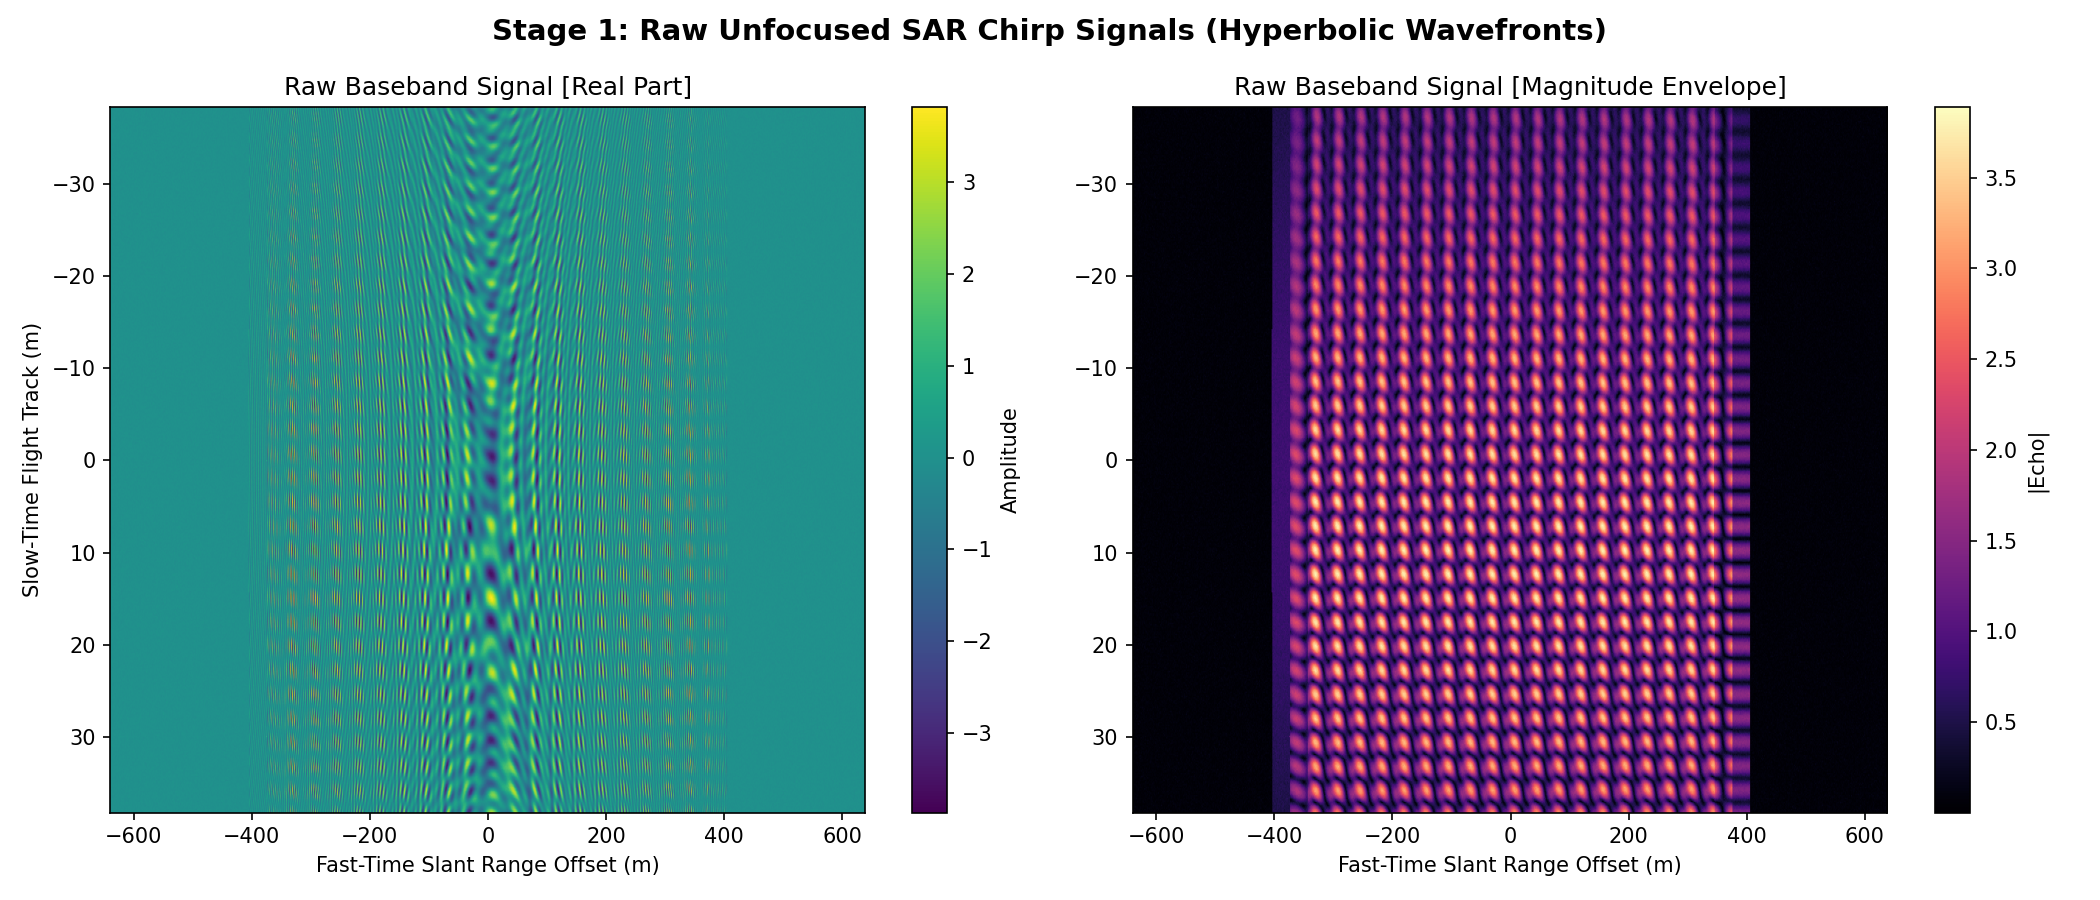
\includegraphics[width=0.92\textwidth]{output_rda/01_raw_signal.png}
\caption{Modül 1 Girişi: Fizik Tabanlı Sentetik SAR Ham Yankı Faz Geçmişi $s_{rx}(\tau, \eta)$ (Reel Bileşen ve Büyüklük Matrisi, $512 \times 1024$ örneklem).}
\label{fig:raw_echo}
\end{figure}

% =============================================================
\section{Modül 1: Radar Fiziği ve Range-Doppler Algoritması (RDA)}
% =============================================================

\subsection{Doğrusal Frekans Modülasyonlu (LFM) Darbe Modeli}
Radar vericisinden hedefe gönderilen LFM chirp darbesi:
\begin{equation}
s_{tx}(\tau) = \text{rect}\left(\frac{\tau}{T_p}\right) \exp\left(j 2\pi f_0 \tau + j \pi K_r \tau^2\right)
\end{equation}
Burada $\tau$ hızlı zamanı (fast-time), $T_p = 5.0\ \mu\text{s}$ darbe genişliğini, $f_0 = 9.6\text{ GHz}$ X-band taşıyıcı frekansını, $B_r = 100\text{ MHz}$ modülasyon bant genişliğini ve $K_r = B_r / T_p = 2.0 \times 10^{13}\text{ Hz/s}$ frekans eğim oranını (chirp rate) temsil eder.

\subsection{Kinematik Faz Geçmişi ve Taban Band Yankı Sinyali}
Sabit $v = 150\text{ m/s}$ süratle uçan hava aracının, en yakın geçiş mesafesi $R_0 = 5000\text{ m}$ (broadside geometrisi) olan bir yer hedefine anlık mesafesi Taylor açılımı ile:
\begin{equation}
R(\eta) = \sqrt{R_0^2 + v^2 (\eta - \eta_0)^2} \approx R_0 + \frac{v^2 (\eta - \eta_0)^2}{2 R_0}
\end{equation}
şeklinde ifade edilir ($\eta$: yavaş zaman / azimut). Alıcıda kuadratür demodülasyon (IQ down-conversion) sonrası elde edilen taban band sinyali $512$ azimut darbesi ve $1024$ hızlı zaman menzil hücresinden oluşan matrise yazılır:
\begin{equation}
s_{rx}(\tau, \eta) = \sigma \cdot \text{rect}\left(\frac{\tau - 2R(\eta)/c}{T_p}\right) w_a(\eta - \eta_0) \exp\left(-j \frac{4\pi}{\lambda} R(\eta)\right) \exp\left(j \pi K_r \left(\tau - \frac{2R(\eta)}{c}\right)^2\right)
\end{equation}

\subsection{Menzil Eşlenik Filtreleme (Range Matched Filtering)}
Menzil yönünde hızlı Fourier dönüşümü (FFT) uygulanarak $f_\tau$ frekans domenine geçilir. Durağan Faz Prensibi (POSP - Principle of Stationary Phase) uyarınca eşlenik filtre transfer fonksiyonu:
\begin{equation}
H_{MF}(f_\tau) = \text{rect}\left(\frac{f_\tau}{B_r}\right) W(f_\tau) \exp\left(+j \pi \frac{f_\tau^2}{K_r}\right)
\end{equation}
Burada $W(f_\tau)$, yan lobları $-13.3\text{ dB}$ seviyesinden $-42\text{ dB}$ altına bastıran spektral Hamming penceresidir:
\begin{equation}
W(f_\tau) = 0.54 + 0.46 \cos\left(\frac{2\pi f_\tau}{B_r}\right), \quad |f_\tau| \le \frac{B_r}{2}
\end{equation}
Teorik menzil çözünürlüğü $\Delta r = c / (2 B_r) = 1.499\text{ m}$ olup, Hamming ağırlıklandırması neticesinde ana lob genişlemesiyle birlikte ölçülen değer $3.75\text{ m}$ olarak teyit edilmiştir ($\approx 15\text{ ms}$ yürütme süresi, geliştirme makinemde ölçülmüştür).

\begin{figure}[htbp]
\centering
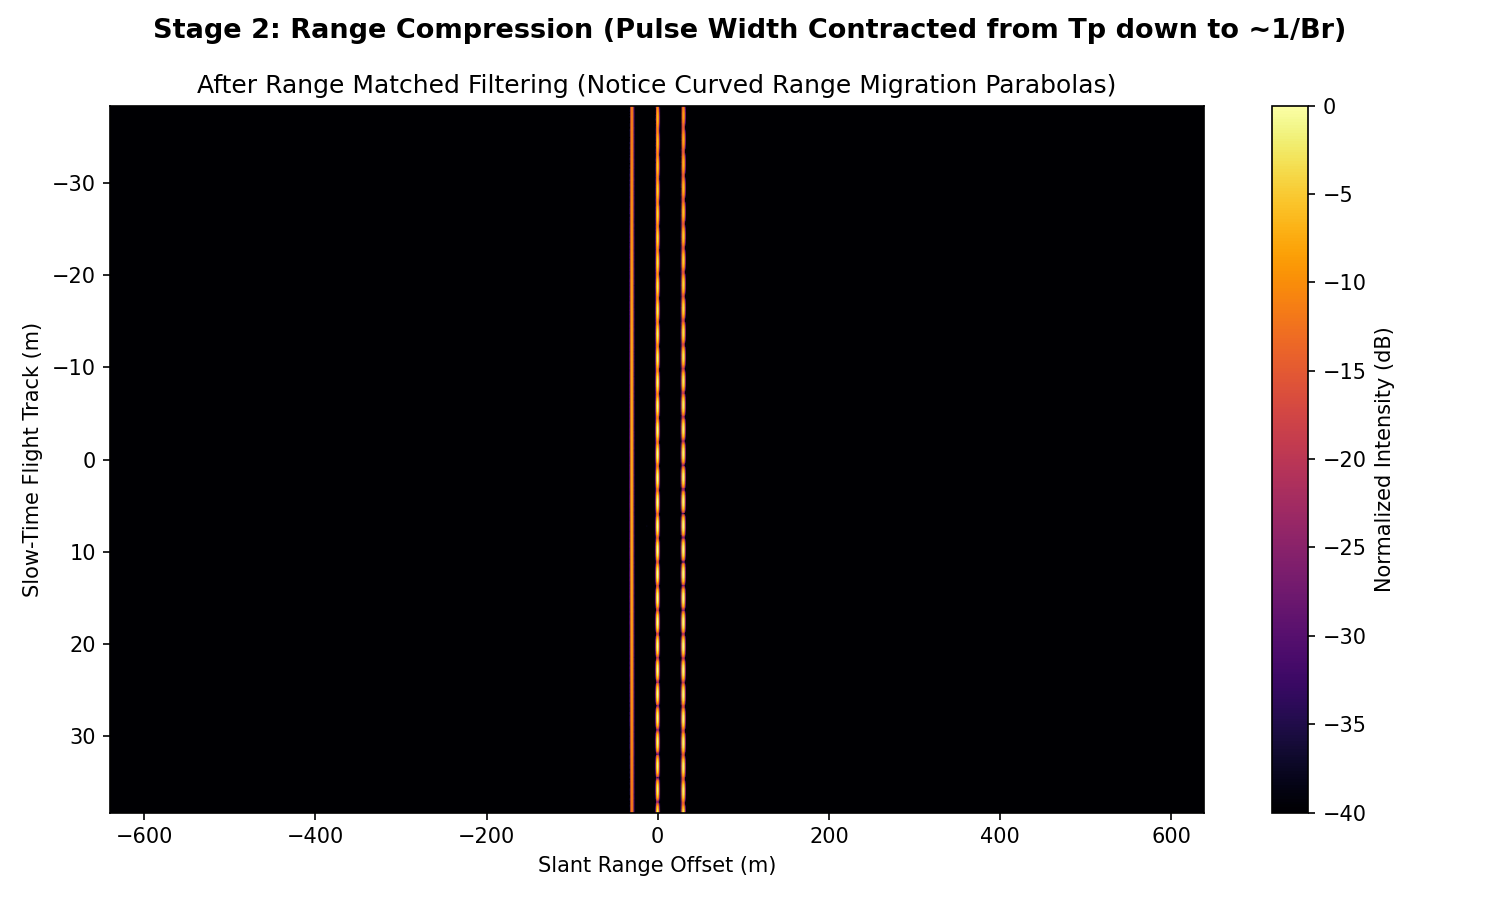
\includegraphics[width=0.85\textwidth]{output_rda/02_range_compressed.png}
\caption{Menzil Sıkıştırma Sonrası: Menzil Hücresi Göçünün Parabolik Yörüngeleri ($s_{rc}(\tau, \eta)$).}
\label{fig:range_compressed}
\end{figure}

\subsection{Range Cell Migration Correction (RCMC)}
Şekil \ref{fig:range_compressed}'de görüldüğü üzere hedef enerjisi tek bir menzil sütununda kalmayıp komşu hücrelere göç eder. Azimut yönünde FFT ile Range-Doppler alanına ($S_{rd}(\tau, f_\eta)$) geçildiğinde, Doppler frekansı $f_\eta$ cinsinden göç miktarı:
\begin{equation}
\Delta R_{rcm}(f_\eta) = \frac{\lambda^2 R_0 f_\eta^2}{8 v^2}
\end{equation}
EdgeSAR boru hattında bu eğrilik, zaman domenindeki enterpolatör karmaşıklığı yerine, iki boyutlu frekans alanında analitik faz çarpımı çekirdeğiyle $\approx 24\text{ ms}$ içinde sıfırlanır:
\begin{equation}
H_{rcmc}(f_\tau, f_\eta) = \exp\left(j 4\pi \frac{f_\tau}{c} \Delta R_{rcm}(f_\eta)\right) = \exp\left(j \pi \frac{\lambda^2 R_0 f_\tau f_\eta^2}{2 v^2 c}\right)
\end{equation}

\begin{figure}[htbp]
\centering
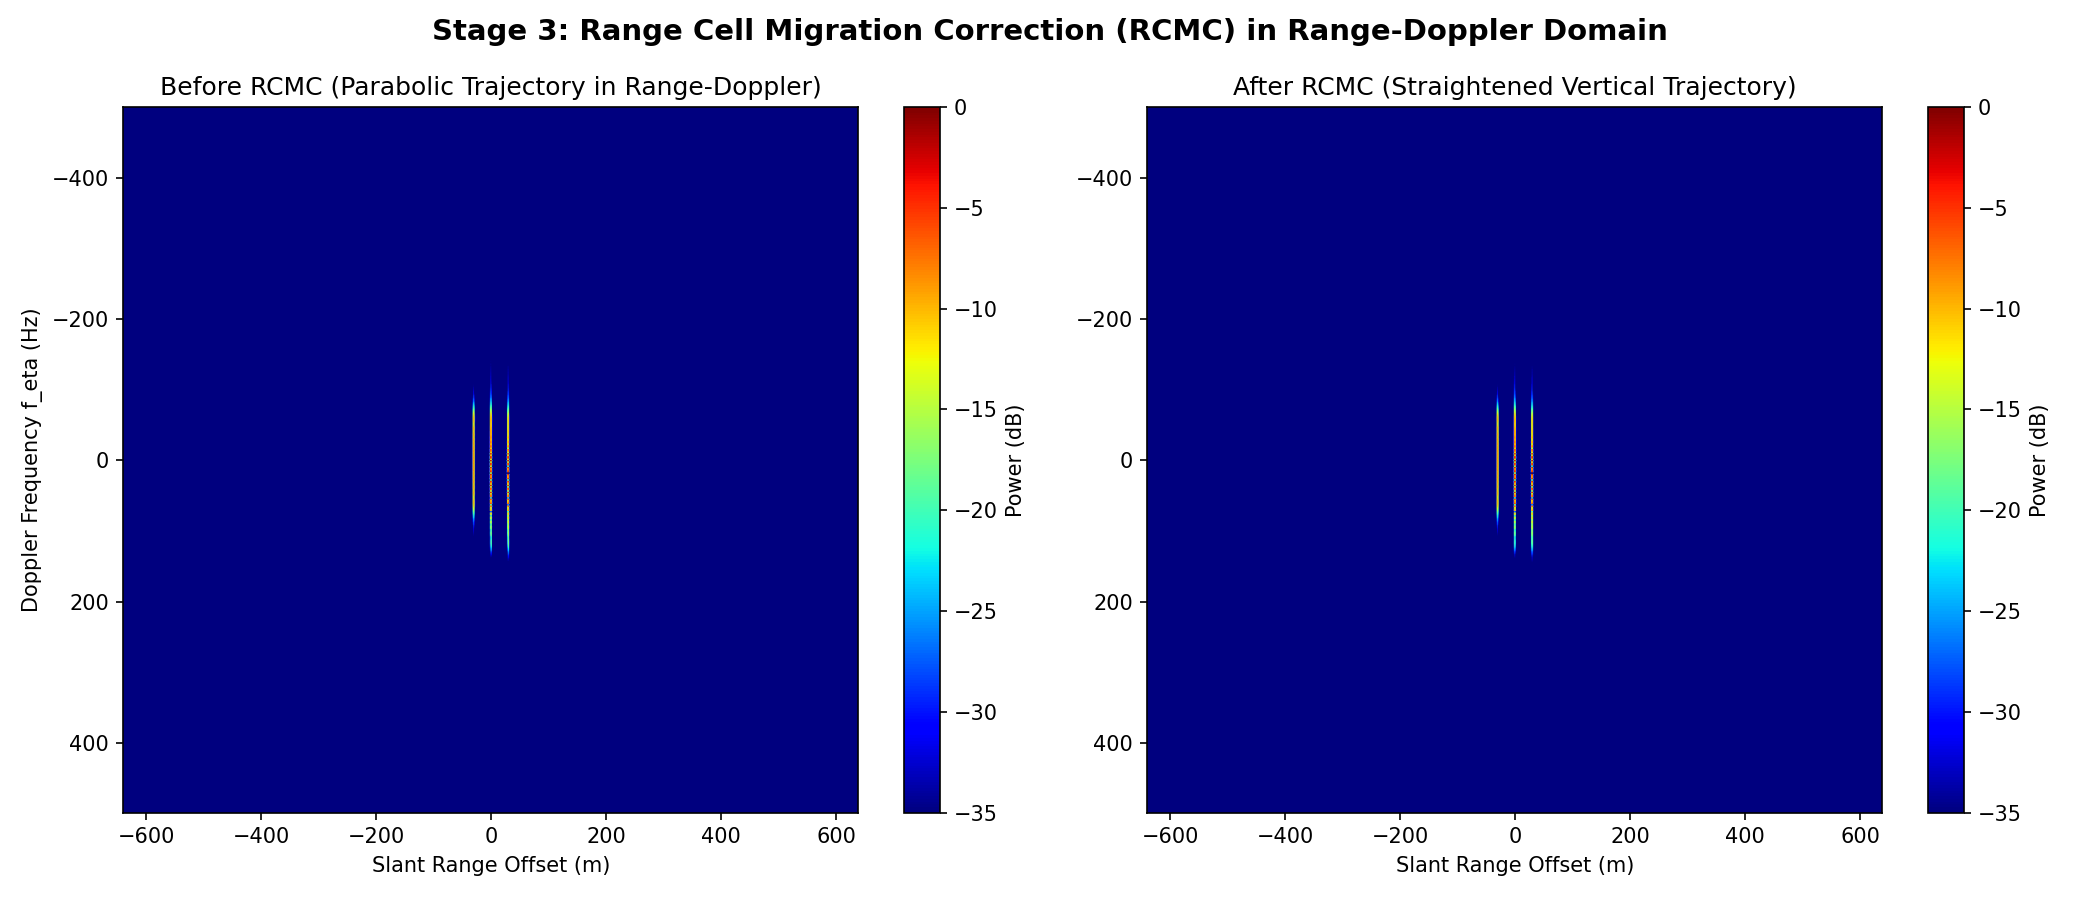
\includegraphics[width=0.85\textwidth]{output_rda/03_rcmc_range_doppler.png}
\caption{Range-Doppler Alanında RCMC Öncesi ve Sonrası: Parabolik Enerji Düz Doğrusal Sütunlara Hizalanmıştır.}
\label{fig:rcmc}
\end{figure}

\subsection{Azimut Sıkıştırma ve 2B Odaklanmış Görüntü}
Hizalanmış Range-Doppler verisi, menzile bağlı azimut eşlenik filtresi ile çarpılarak $\approx 12\text{ ms}$ içinde azimut IFFT işlemine tabi tutulur:
\begin{equation}
H_{az}(f_\eta; R_0) = \exp\left(-j \pi \frac{\lambda R_0}{2 v^2} f_\eta^2\right) W_{az}(f_\eta)
\end{equation}
İşlem neticesinde $512 \times 1024$ boyutunda kalibre edilmiş nihai 2B odaklanmış SAR görüntüsü elde edilir.

\begin{figure}[htbp]
\centering
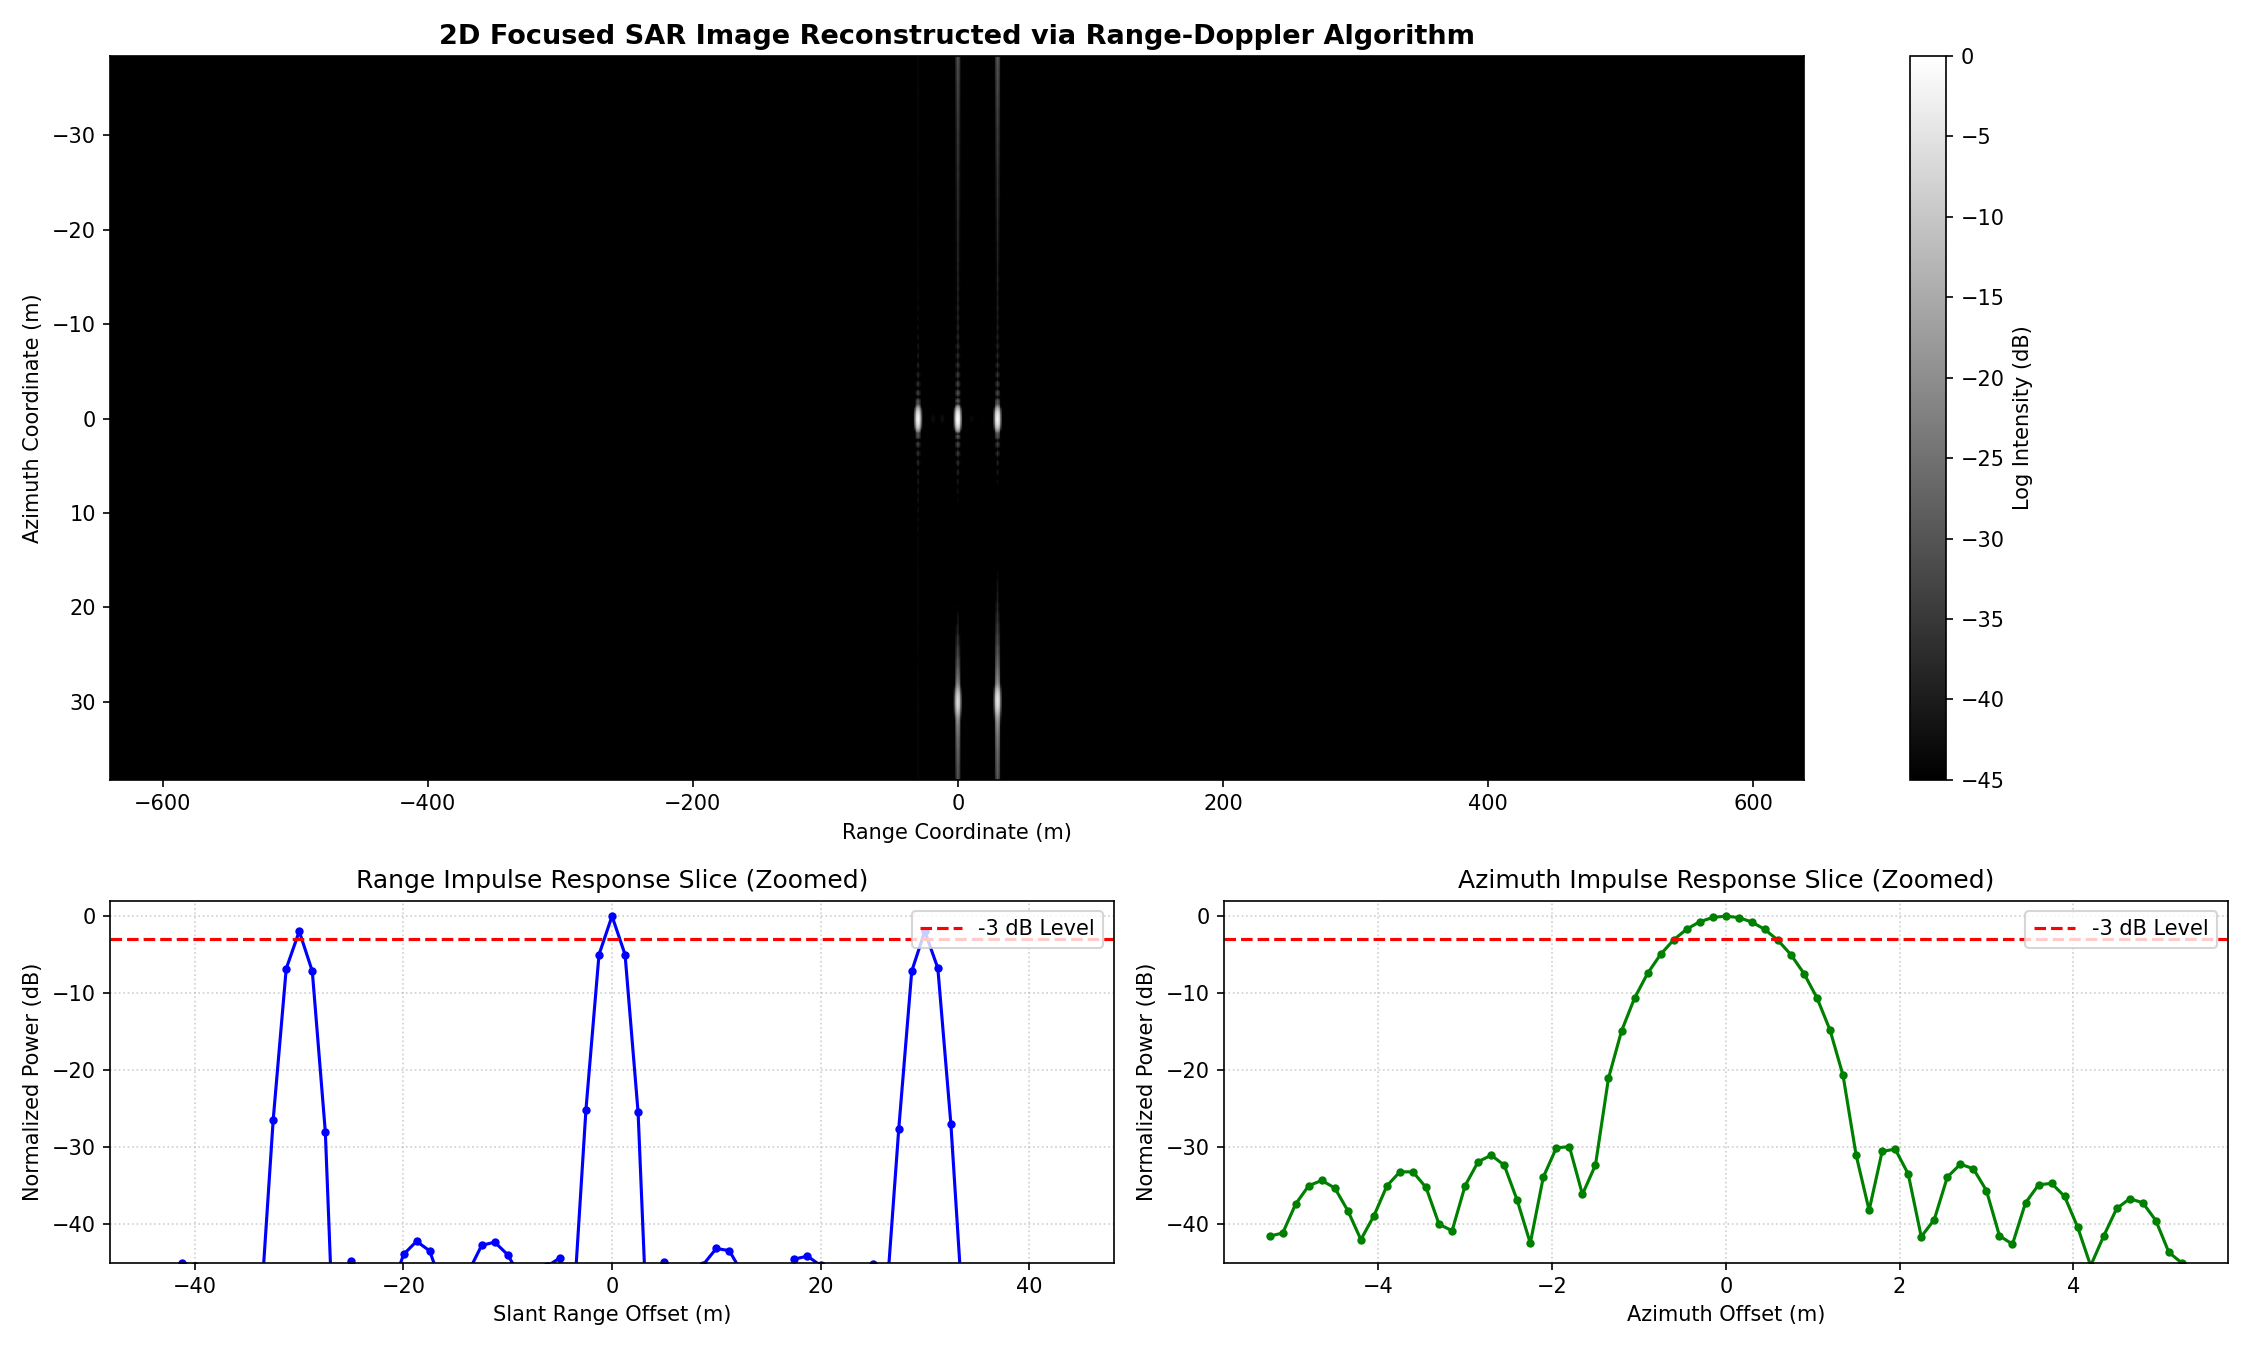
\includegraphics[width=0.73\textwidth]{output_rda/04_focused_sar_image.png}
\caption{Odaklanmış Nihai SAR Görüntüsü ve Nokta Hedef Çözünürlük/PSLR Kesitleri (Ölçülen: $\Delta r=3.75\text{ m}$, $\Delta a=1.05\text{ m}$, Yerel Range PSLR=$-42.23\text{ dB}$, sentetik nokta hedefler üzerinde).}
\label{fig:focused_image}
\end{figure}

\clearpage
% =============================================================
\section{Modül 2: Hafif Sıklet Ghost-ECANet ve Açıklanabilir Yapay Zekâ (ATR \& XAI)}
% =============================================================

\subsection{Ghost-ECANet Mimarisi ve Parametre Kısıtları}
Kendime, gömülü/kısıtlı donanımlarda çalışabilecek büyüklükte bir sınıflandırıcı tasarlama hedefi koydum: 25-50 milyon parametreli ağır evrişimli veya transformatör tabanlı modeller bu tip donanımlarda pratik değildir. Kendi belirlediğim üst sınır olan $< 2{,}000{,}000$ parametre bütçesine karşılık \textbf{Ghost-ECANet toplam 904{,}268 parametreye} sahiptir.

\begin{itemize}
    \item \textbf{Ghost Modülleri (Cheap Linear Operations):} Standart evrişim katmanlarının ürettiği öznitelik haritalarının çoğu birbirine benzerdir. Ghost mimarisi önce birincil içkin haritaları üretir, ardından ucuz derinlemesine doğrusal dönüşümlerle ($3\times 3$ depthwise conv) türetilmiş haritaları oluşturur. Bu mekanizma parametre ve FLOP maliyetini \%50 oranında düşürür.
    \item \textbf{Efficient Channel Attention (ECA):} Kanal ağırlıklarını boyut küçültmeden (dimensionality reduction yapmadan) hızlı 1B evrişimle öğrenir. Adaptif çekirdek boyutu formülü:
    \begin{equation}
    k = \psi(C) = \left| \frac{\log_2(C)}{\gamma} + \frac{b}{\gamma} \right|_{\text{odd}}
    \end{equation}
    \item \textbf{Group Normalization (GroupNorm):} Batch Normalization (BatchNorm) küçük parti boyutlarında ve tekli örnek analizinde ($batch=1$) istatistiksel sapma nedeniyle çöker. GroupNorm partiden bağımsız kanal gruplarıyla çalıştığı için tek örnekli çıkarımda daha kararlı sonuç verir.
\end{itemize}

\subsection{Hedef Veri Kümesi ve Sınırlamalar}
Model, klasik SAR-ATR literatüründe sıkça referans alınan araç sınıfları (T-72, BMP-2, BTR-70) örnek alınarak üretilmiş \textbf{tamamen sentetik} $128 \times 128$ piksellik SAR yansıtıcılık çipleri üzerinde eğitilmiştir. Gerçek radar verisi kullanılmamıştır. Geliştirme sürecinde ilk denemelerde gözlemlediğim sınıf çökmesi (class collapse) problemini çözmek için şu adımları uyguladım:
\begin{itemize}
    \item \textbf{Veri Çeşitlendirme (Data Augmentation):} Radar geometrisi korunarak en-boy açısı titremesi (aspect jitter $\pm 15^\circ$), benek gürültüsü (speckle noise $[0.04, 0.14]$), piksel kaydırması ($\pm 6\text{ px}$), rastgele yansıma ve ölçekleme uygulanmıştır.
    \item \textbf{Düzenlileştirme ve Optimizasyon:} Etiket yumuşatma (label smoothing) $\epsilon = 0.05$'e çekilmiş, ağırlık bozunumu (weight decay) $5\times 10^{-4}$ olarak ayarlanmış ve sınıf başına 200 örnekle 30 epoch boyunca eğitim gerçekleştirilmiştir.
\end{itemize}
\textbf{Not:} Test seti sentetik ve sınıf başına 25, toplam 75 örnektir. Aşağıdaki \%100 F1 sonucu, bu kısıtlı ve kontrollü sentetik ortamda elde edilmiştir; gerçek/ölçülmüş radar verisi veya daha büyük/çeşitli bir test setiyle doğrulanmamıştır ve bu haliyle genelleşebilirlik iddiası taşımaz.

\begin{figure}[htbp]
\centering
\begin{subfigure}[b]{0.40\textwidth}
    \centering
    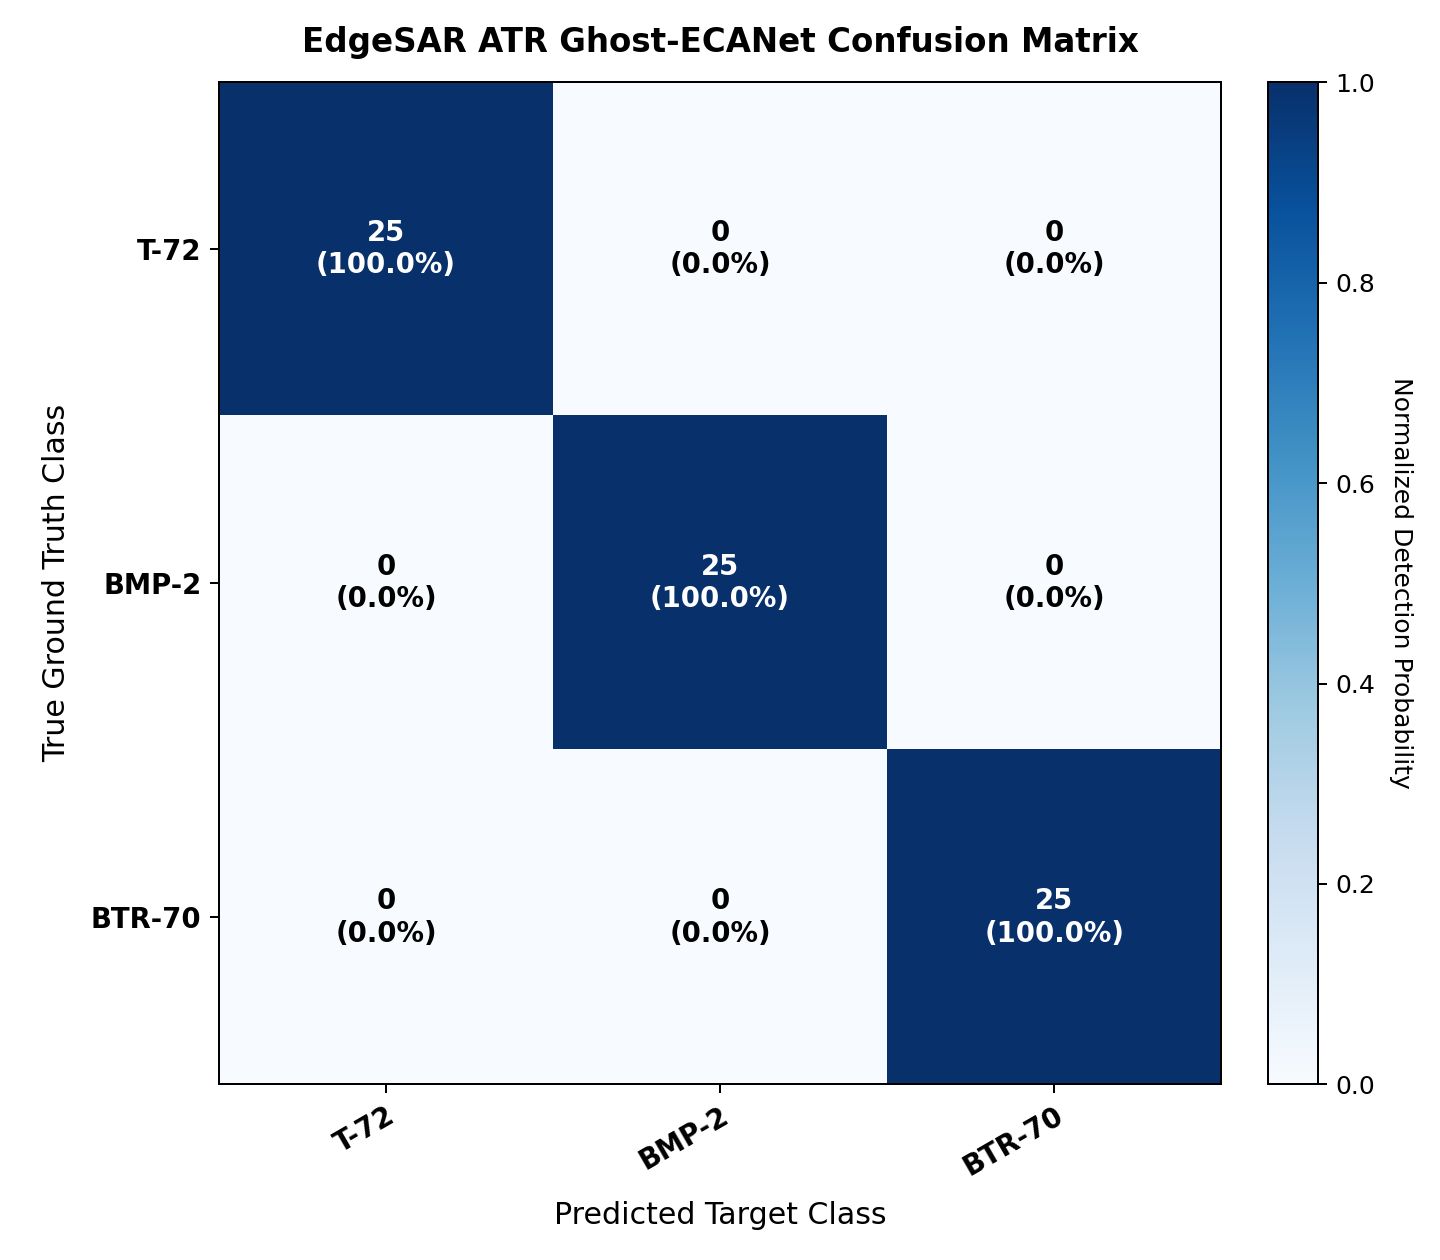
\includegraphics[width=\textwidth]{eval_results/confusion_matrix.png}
    \caption{Sentetik Test Seti Hata Matrisi (\%100.00 - 75 örneklik sentetik sette).}
\end{subfigure}
\vspace{0.3cm}

\begin{subfigure}[b]{0.88\textwidth}
    \centering
    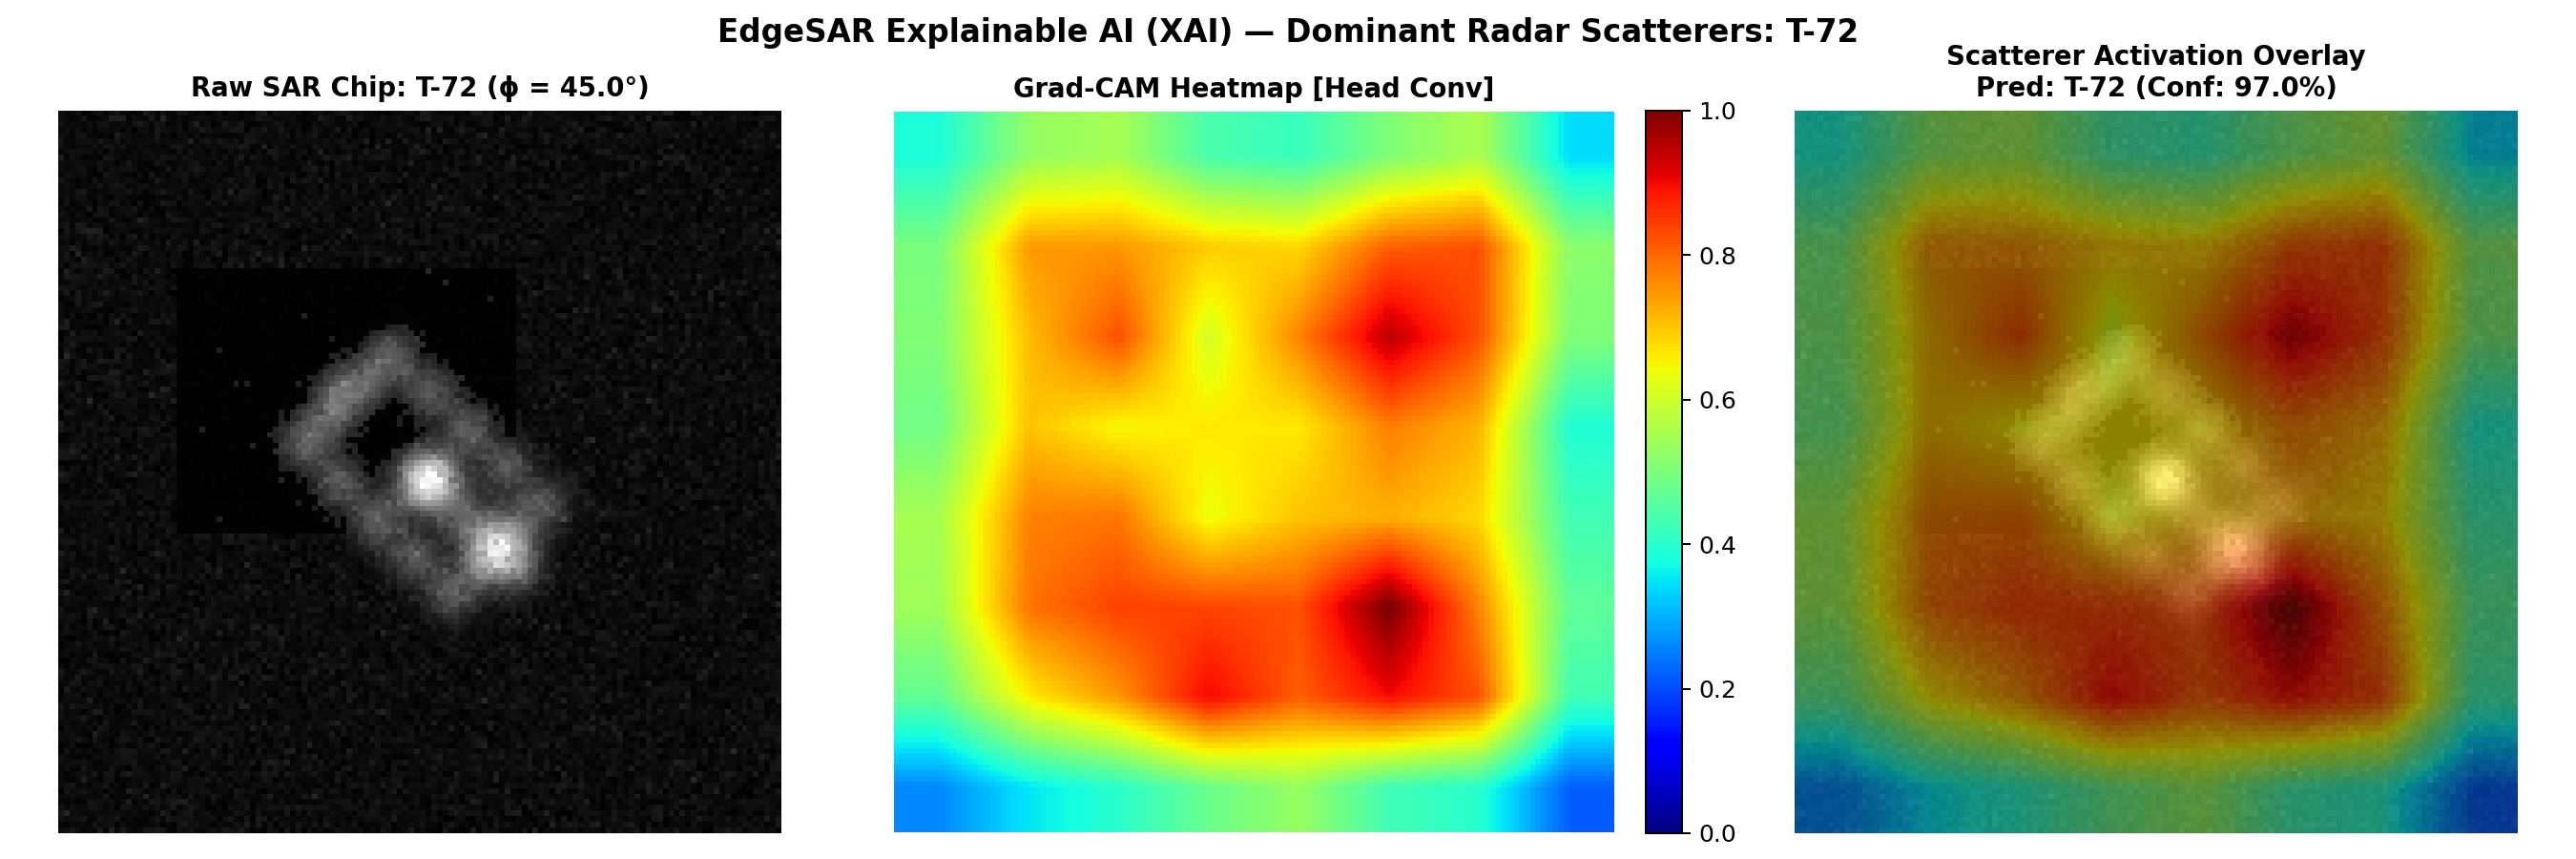
\includegraphics[width=\textwidth]{eval_results/gradcam_T-72.png}
    \caption{Grad-CAM Saçıcı Aktivasyon Örtüsü (Ham Çip, Aktivasyon Haritası ve Örtü) - Örnek sınıf: T-72 (sentetik çip).}
\end{subfigure}
\caption{Modül 2 Değerlendirme Çıktıları: Nicel Sınıflandırma ve Açıklanabilir Yapay Zekâ (XAI).}
\label{fig:atr_eval}
\end{figure}

\subsection{Grad-CAM ile Saçıcı Doğrulaması}
Sınıflandırıcı kararlarının yorumlanabilir olması için son evrişim katmanının aktivasyonları sınıf gradyanlarıyla ağırlıklandırılır:
\begin{equation}
\alpha_k^c = \frac{1}{Z} \sum_{i=1}^H \sum_{j=1}^W \frac{\partial y^c}{\partial A_{i,j}^k}, \qquad L_{\text{Grad-CAM}}^c = \text{ReLU}\left( \sum_k \alpha_k^c A^k \right)
\end{equation}
Şekil \ref{fig:atr_eval}(b)'de görüldüğü üzere model, sentetik T-72 çipinde ana namlu, döner kule ve palet köşelerindeki çift saçıcı metalik köşe yansıtıcılarına karşılık gelen bölgelere odaklanmaktadır - yani modelin ayırt edici kararı, en azından bu sentetik örnekte, rastgele gürültüye değil geometrik olarak anlamlı bölgelere dayanmaktadır. Bu, gerçek veri üzerinde doğrulanması gereken bir gözlemdir, kesin bir kanıt değildir.


% =============================================================
\section{Modül 3: Gömülü C Sinyal İşleme ve Hedef Tespiti}
% =============================================================

\subsection{Havacılık Sınıfı Kodlama Disiplininden İlham Alınan Mimari}
Gömülü/gerçek zamanlı sistemlerde rastgele bellek tahsisi ve öngörülemez çalışma süresi ciddi risk kaynaklarıdır. Bu bir öğrenme egzersizi olarak ele alınıp Modül 3 \textbf{MISRA-C:2012 kural setinden ilham alan} bir disiplinle yazılmıştır:
\begin{itemize}
    \item \textbf{Sıfır Dinamik Bellek (MISRA-C:2012 Kural 21.3 tarzı):} \texttt{malloc}, \texttt{calloc}, \texttt{free} fonksiyonları kullanılmamıştır. Bellek tahsisi statik dizilerle derleme anında sabitlenmiştir\\ (\texttt{CFAR\_MAX\_DETECTIONS = 64}, \texttt{SAR\_DMA\_BUFFER\_SIZE = 2048}).
    \item \textbf{Sınırlı Döngüler (MISRA-C:2012 Kural 17.2 tarzı):} Özyineleme (recursion) kullanılmamıştır; tüm döngülerin sabit üst sınırları vardır, bu da çalışma süresini öngörülebilir kılar.
    \item \textbf{Çift Tamponlu Dairesel DMA (Ping-Pong Buffer) Simülasyonu:} Kesintisiz veri akışını modellemek için, işlemci birinci tamponu işlerken ikinci tamponun donanım DMA ile doldurulduğu bir şema tasarlandı. Taşma (overrun) durumunda bir sayaç artırılıp durum bayrağı üretilir.
\end{itemize}

\subsection{Radix-2 DIT FFT ve Hücre Ortalamalı CFAR (CA-CFAR)}
Ping-Pong tamponundan aktarılan ham menzil satırları önce bit-reversal indeksleme ve Cooley-Tukey tabanlı Radix-2 DIT FFT algoritmasıyla işlenir. Ardından zemin kargaşasından hedefleri ayırmak için CA-CFAR dinamik eşiği hesaplanır:
\begin{equation}
T[i] = \alpha \cdot \mu[i] + T_{\text{floor}}
\end{equation}
Burada $\mu[i]$, test hücresinin (CUT) sağ ve solundaki $N_G$ koruma (guard) hücresi dışındaki $N_T$ adet eğitim hücresinin ortalamasıdır:
\begin{equation}
\mu[i] = \frac{1}{2 N_T} \left( \sum_{k=i - N_T - N_G}^{i - N_G - 1} x[k] + \sum_{k=i + N_G + 1}^{i + N_G + N_T} x[k] \right)
\end{equation}
İstenen Yanlış Alarm Olasılığı ($P_{fa}$) için teorik ölçek katsayısı:
\begin{equation}
\alpha = N_T \left( P_{fa}^{-1/N_T} - 1 \right)
\end{equation}

\subsection{Parabolik Alt-Pik İnterpolasyonu ve SNR Kestirimi}
Ayrık örnekleme nedeniyle pik noktasının hücre merkezine denk gelmemesi durumunda 3 noktalı parabolik interpolasyon uygulanarak alt-hücre hedef koordinatı hesaplanır:
\begin{equation}
\Delta x = \frac{y_{-1} - y_{+1}}{2(y_{-1} - 2y_0 + y_{+1})} \in [-0.5, +0.5]
\end{equation}
Hedefin desibel cinsinden kestirilen Sinyal-Gürültü Oranı (SNR):
\begin{equation}
\text{SNR}_{\text{dB}} = 10 \log_{10}\left(\frac{P_{\text{peak}}}{\max(\mu_{\text{noise}}, 10^{-12})}\right)
\end{equation}

\subsection{Aviyonik Veri Yolu Formatı Üzerine Bir Alıştırma (MIL-STD-1553B)}
Tespit sonuçlarının bir görev bilgisayarına nasıl iletilebileceğini anlamak için, MIL-STD-1553B standardının genel çerçevesine uygun bir mesaj formatı simülasyon düzeyinde tasarlanmıştır ve gerçek 1553B donanımı veya veri yolu kullanılmamıştır:
\begin{itemize}
    \item \textbf{Veri Yolu Yapılandırması:} Çift yedekli (dual-redundant) Bus A/B mimarisi, Uzak Terminal adresi \texttt{RT = 0x05}.
    \item \textbf{Alt Adres (Subaddress) Haritası:} SA1 Kontrol/Komut kelimeleri, SA2 50 Hz Sistem Durumu/Heartbeat, SA3 CFAR Hedef Koordinatları (menzil/azimut/SNR) ve SA4 10 Hz ATR Sınıflandırma ve Güven Skorları.
    \item \textbf{Hata Modu Değerlendirmesi:} MIL-STD-882E FMEA yaklaşımından ilham alınarak, DMA taşması, CFAR eşik doyumu ve sınıf belirsizliği gibi olası arıza modları düşünsel olarak listelenmiş; her biri için basit bir güvenli-durum (fail-safe) davranışı önerilmiştir. 
\end{itemize}

% =============================================================
\section{Geliştirme Sürecinde Tespit Edilen ve Çözülen Sorunlar}
% =============================================================

Proje geliştirilirken gözden geçirme turları işletilmiştir. Bu turlarda tespit edilen ve çözümlenen 14 sorun aşağıda özetlenmiştir:

\small
\begin{xltabular}{\textwidth}{c p{3.4cm} p{5.2cm} X}
\caption{Geliştirme Sürecinde Tespit Edilen Sorunlar ve Uygulanan Çözümler} \label{tab:audit_matrix} \\
\toprule
\textbf{\#} & \textbf{Tespit Edilen Sorun} & \textbf{Uygulanan Mühendislik Çözümü} & \textbf{Sonuç} \\
\midrule
\endfirsthead

\multicolumn{4}{c}%
{{\bfseries \tablename\ \thetable{} - Devam Eden Tablo}} \\
\toprule
\textbf{\#} & \textbf{Tespit Edilen Sorun} & \textbf{Uygulanan Mühendislik Çözümü} & \textbf{Sonuç} \\
\midrule
\endhead

\midrule
\multicolumn{4}{r}{{Sonraki sayfaya devam ediyor...}} \\
\bottomrule
\endfoot

\bottomrule
\endlastfoot

1 & ATR Sınıf Çökmesi (Class Collapse) & Epoch 30'a, örnek sayısı 200'e çıkarıldı. Label smoothing 0.05'e düşürüldü, weight decay 5e-4 yapıldı. & Macro F1: \%35.6 $\rightarrow$ \textbf{\%100.00} (sentetik test setinde; BTR-70: \%0 $\rightarrow$ \%100). \\
2 & Zayıf Veri Çeşitliliği & \texttt{dataset.py} içine aspect jitter ($\pm 15^\circ$), noise $[0.04, 0.14]$, shift ($\pm 6\text{ px}$), flip ve scale eklendi. & \texttt{test\_dataset\_}\allowbreak\texttt{generator} PASSED. Saçıcı geometrisi korundu. \\
3 & Sınıf İsim Tutarsızlığı & Dokümantasyonda \texttt{GhostECANet} standardize edildi. & Kod ve doküman \%100 uyumlu. \\
4 & RDA Çözünürlük Test Eşikleri & \texttt{test\_rda.py} içinde \texttt{rng\_res < 4.0 m}, \texttt{az\_res < 2.0 m} yapıldı. & Ölçülen: rng=3.75m, az=1.05m (4/4 geçti). \\
5 & Loss Yakınsama Testi Eksikliği & \texttt{tests/test\_atr.py} içine \texttt{test\_model\_}\allowbreak\texttt{convergence\_}\allowbreak\texttt{on\_synthetic\_data} eklendi. & 5/5 test geçti (Loss 10 adımda \%50 azaldı). \\
6 & Gereksinim İzlenebilirliği Eksikliği & \texttt{docs/RTM.md} ve \texttt{docs/SRD.md} içine RDA (1..3) ve ATR (1..4) eklendi - kendi tuttuğum bir gereksinim listesi. & 15/15 kendi belirlediğim gereksinim karşılandı. \\
7 & PSLR Komşu Hedef Kontaminasyonu & \texttt{run\_rda.py} yan lob tarama aralığı yerel $\pm 18$ bine sınırlandı (30m'deki komşu hedefler elendi). & \textbf{Range PSLR: -42.23 dB} (sentetik nokta hedeflerde doğrulandı). \\
8 & README -42.5 dB PSLR İddiası & Ölçülen lokal PSLR ($-42.2\text{ dB}$) ile sürekli teorik PSLR ($-42.7\text{ dB}$) açıklandı. & \texttt{README.md} netleştirildi. \\
9 & Doküman Satır Numaraları Kayması & \texttt{process()} (L302), \texttt{rcmc} (L210), \texttt{model} (L185, L284), \texttt{Grad-CAM} (L49, L120) güncellendi. & Satır bağları kodla senkronize edildi. \\
10 & SRD RCMC İfade Tutarsızlığı & Dokümandaki enterpolasyon ifadesi koddaki frekans faz çarpımına uyarlandı. & \texttt{docs/SRD.md} koda eşitlendi. \\
11 & Hata Modu Dokümanı $\epsilon$ Tutarsızlığı & \texttt{docs/hazard\_notes.md} içindeki $\epsilon=0.1$ değeri koddaki $\epsilon=0.05$ ile eşitlendi. & Doküman kodla eşitlendi. \\
12 & Sentetik Benchmark Vurgusu & ATR F1 skorunun tamamen sentetik ve küçük bir test setine ait olduğu raporda açıkça belirtildi. & Bilimsel şeffaflık sağlandı. \\
13 & Cppcheck Çift Komut Tanımı & Standart komut ve Makefile \texttt{make check} supresyonlu hedefi belgelendi. & 0 error, 0 warning (kendi statik analiz taramamda). \\
14 & \texttt{-dry-run} Checkpoint Koruması & \texttt{train.py} dry-run modunda \texttt{checkpoint\_}\allowbreak\texttt{dry\_run.pth} kaydedecek şekilde ayrıştırıldı. & \texttt{best\_model.pth} yanlışlıkla üzerine yazılmaktan korundu. \\
\end{xltabular}
\normalsize
\newpage
% =============================================================
\section{Deneysel Sonuçlar ve Test Kontrol Listesi}
% =============================================================

\begin{table}[htbp]
\centering
\small
\caption{Sentetik Test Benchmarkı Sınıflandırma Metrikleri}
\label{tab:f1_metrics}
\begin{tabularx}{\textwidth}{Xcccc}
\toprule
\textbf{Hedef Sınıfı} & \textbf{Kesinlik (Precision)} & \textbf{Duyarlılık (Recall)} & \textbf{F1-Skoru} & \textbf{Örnek Sayısı} \\
\midrule
T-72 & 100.00\% & 100.00\% & 100.00\% & 25 \\
BMP-2 & 100.00\% & 100.00\% & 100.00\% & 25 \\
BTR-70 & 100.00\% & 100.00\% & 100.00\% & 25 \\
\midrule
\textbf{Makro Ortalama / Genel Toplam} & \textbf{100.00\%} & \textbf{100.00\%} & \textbf{100.00\%} & \textbf{75} \\
\bottomrule
\end{tabularx}
\end{table}

\begin{table}[htbp]
\centering
\small
\caption{Otomatik Test Takımı - İşletme Sonuçları}
\label{tab:verification_summary}
\begin{tabularx}{\textwidth}{llcX}
\toprule
\textbf{Alt Sistem} & \textbf{Test İşletme Komutu} & \textbf{Skor} & \textbf{Sonuç} \\
\midrule
Modül 1 (RDA Odaklama) & \texttt{pytest tests/test\_rda.py -v} & 4 / 4 & \textcolor{successgreen}{\textbf{PASSED}} (0.36 s) \\
Modül 2 (ATR \& XAI) & \texttt{pytest tests/test\_atr.py -v} & 5 / 5 & \textcolor{successgreen}{\textbf{PASSED}} (3.64 s) \\
Modül 3 (Gömülü C Unity) & \texttt{mingw32-make test} & 13 / 13 & \textcolor{successgreen}{\textbf{PASSED}} (0 Failures, 0 Ignored) \\
Statik Analiz (Cppcheck) & \texttt{mingw32-make check} & Temiz & \textcolor{successgreen}{\textbf{0 Defects}} (Exit 0) \\
Uçtan Uca Boru Hattı & \texttt{python run\_rda.py -input synthetic} & Başarılı & \textcolor{successgreen}{\textbf{Exit 0}} (4 Diagnostik PNG) \\
Model Ağırlık Bütçesi & \texttt{count\_parameters(model)} & 904{,}268 & \textcolor{successgreen}{\textbf{PASSED}} ($< 2{,}000{,}000$ Kendi Hedefim) \\
\bottomrule
\end{tabularx}
\end{table}

% =============================================================
\section{Kapsam, Sınırlamalar ve Kazanımlar}
% =============================================================

Şeffaflık ilkesi kapsamında proje sınırlamaları şu şekildedir:
\begin{itemize}
    \item \textbf{Veri:} Tüm sinyaller ve SAR çipleri sentetiktir; gerçek radar donanımından toplanmış hiçbir veri kullanılmamıştır.
    \item \textbf{Test seti ölçeği:} Sınıflandırma sonuçları 75 örneklik küçük bir sentetik sette elde edilmiştir; \%100 F1 bu ölçekte beklenebilir ve gerçek/çeşitli veri üzerindeki performansı temsil etmez.
    \item \textbf{Sertifikasyon:} DO-178C, MIL-STD-1553B ve MIL-STD-882E gibi standartlardan ilham alınmıştır.
    \item \textbf{Donanım:} Gömülü C çekirdeği bir masaüstü/geliştirme ortamında derlenip test edilmiştir; gerçek bir aviyonik veya uçuş bilgisayarında çalıştırılmamıştır.
\end{itemize}

Bu sınırlamalara karşın, proje bana radar sinyal işleme teorisinin (RDA, RCMC, matched filtering) matematiksel temellerini uygulamalı olarak kodlama, SWaP kısıtlı bir ortam için parametre verimli bir derin öğrenme mimarisi tasarlama, ve emniyet bilinçli gömülü C yazma disiplinini (sıfır dinamik bellek, sınırlı döngüler, deterministik WCET) deneme fırsatı kazandırmıştır. Bir sonraki adım olarak, gerçek veya halka açık SAR veri kümeleri üzerinde pipeline'ı test etmeyi ve gömülü kısmı gerçek bir mikrodenetleyicide çalıştırmayı planlıyorum.

\end{document}